\documentclass[a4paper,12pt,twoside]{article}
\usepackage[T1]{fontenc}
\usepackage[utf8]{inputenc}
\usepackage{lmodern}
\usepackage{url,csquotes}
\usepackage[hidelinks,hyperfootnotes=false]{hyperref}
\usepackage[titlepage,pagenumber]{polytechnique}
\usepackage{float}

\title{MAP-536 - Python for Data Science}
\subtitle{Final Project - Air data prediction}
\author{Leonardo \textsc{Natale} \& Guillaume \textsc{Le Fur}}
\logo{scikit_learn.jpeg}

\begin{document}

\maketitle

\section{External Data and Data Preprocessing}

\subsection{Getting External Data}
The original data consists of : The date of departure, the departure and arrival airport, the mean and standard deviation of the number of weeks of the reservations made before the departure date, a field called log\_PAX which is related to the number of passengers (the actual number were changed for privacy reasons).

We have added the following data:
\begin{itemize}
	\item Daily Jet Fuel Price
	\item Airport Location (geographical coordinates)
	\item Departure and Arrival GDP
	\item Monthly flow of passengers in the US between airports.
	\item Daily Weather Data
	\item US Holiday Calendar
\end{itemize}

\subsection{Feature Engineering}

We were able to add the following extra features, by using the data described above:
\begin{itemize}
	\item Number of days to the closest holiday.
	\item Distance in kilometers between departure and arrival airport.
	\item Airport Dimension
	\item Monthly log\_PAX per airport, both arrival and departure.
\end{itemize}


\section{Structure}
(Adjust the size and position, maybe explanation at the right)
\begin{figure}[H]
	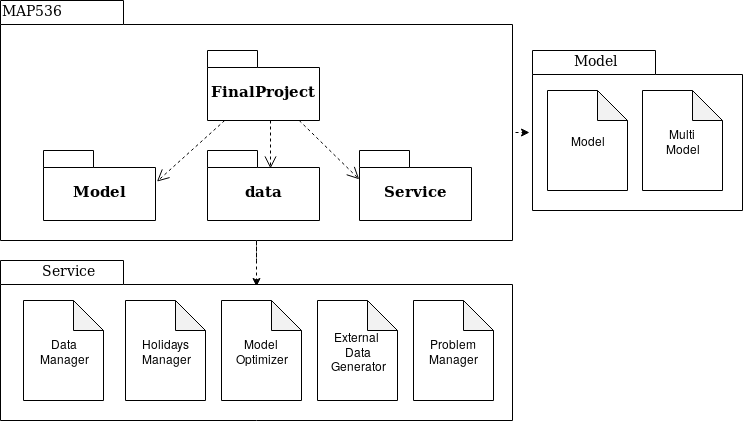
\includegraphics[width=100mm,scale=0.5]{UML.png}
\end{figure}

\begin{itemize}
	\item \textbf{Data} contains all the external data files that we use to create our additional features.
	\item \textbf{ExtrnalDataGenerator} merges all our external data into the \textit{external_data.csv} file. It is the class that is responsible for all the feature engineering of our models.
	\item \textbf{DataManager} is some kind of an interface between the model and the external data. It takes data as an input (either the train or test data) and merges it with external data, making it ready for fitting.
	\item \textbf{Model} is a utility class that stores a sklearn model and two lists : a list of parameters that are to optimize via GridSearchCV and another with parameters that are to be optimized via RandomSearchCV. The main role of this class, when used locally, is to compare the quality of the fit of a model before and after optimization of the hyper-parameters. When used on RAMP, it's role is to contain the model and to fit and predict based on the data passed as an input.
	\item \textbf{MultiModel} is a class that goal is to simplify the testing of multiple models at the same time. When creating an instance, one can pass multiple models and hyper-parameters list. Then all the models are going to be optimized. The predict method can be used in two different ways : either returning separate predictions for each model or either making the average of the models, which can allow to test models that are combinations of several models.
	\item \textbf{ModelOptimizer} is an interface, called by Model, that takes care of the RandomSearchCV and GridSearchCV and returns the result to model.
	\item \textbf{HolidaysManager} is a utility class used to vectorize operations on dates to determine whether they are holidays or how close they are to a holiday.
	\item \textbf{ProblemManager} is a class that contains metadata about the problem we intend to solve (columns that are relevant, external data we use, etc.)
\end{itemize}

\section{Models and Tuning}
\subsection{Models}
Add a table with comparison between different models.
\begin{center}
	\begin{tabular}{||c || c c c||} 
		\hline
			 & Train RMSE & Test RMSE & Train time (s) \\ [0.5ex] 
		\hline\hline
		\textbf{Model1} & 6 & 87837 & 787 \\ 
		\hline
		\textbf{Model2} & 7 & 78 & 5415 \\
		\hline
		\textbf{Model3} & 545 & 778 & 7507 \\
		\hline
	\end{tabular}
\end{center}
Explain why we have chosen our model.

\subsection{Hyperparameters Tuning}
Our ModelOptimizer class is in charge of the optimization of the models by Grid Search and Randomized Search. It is composed by two methods:
\begin{itemize}
	\item grid\_search\_optimize runs a GridSearchCV with the given params and outputs the optimal value of the parameters for the model.
	\item random\_search\_optimize runs a a RandomSearchCV with the given params to which we associate the given distribution.
\end{itemize}

\section{Conclusion}
\subsection{Model Interpretability}
Feature importance graph and comments.
\subsection{Evaluation of Uncertainty in Predictions}
Talk about: 
\subsection{Final Comments and Possible Improvements}

\end{document}
